\section{Durchführung}
\label{sec:Durchführung}
\begin{figure}[h!]
	\centering
	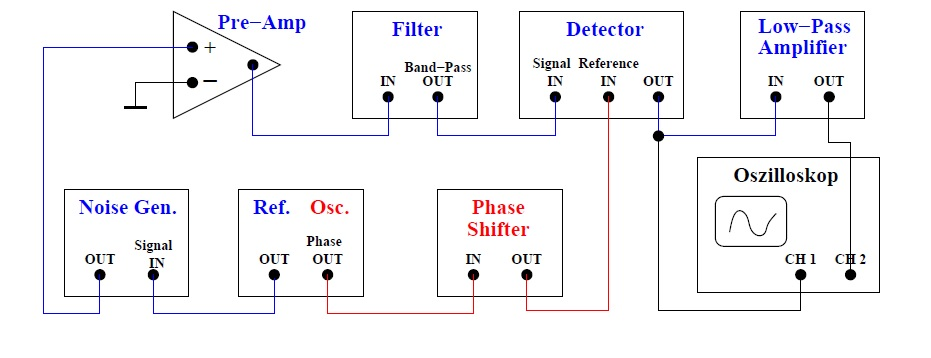
\includegraphics[width=0.8\linewidth]{aufbau1.jpg}
	\caption{Aufbau des verwendeten Lock-In-Verstäkers im ersten Versuchsteil. \cite[3]{anleitung303} }
	\label{fig:aufbau1}
\end{figure}

Die verwendete Messaparatur ist modular in der Abbildung \ref{fig:aufbau1} aufgebaut. Damit können die Komponenten einzeln untersucht werden und der Lock-In-Verstärker kann Schritt für Schritt aufgebaut werden. 
Zu bedienen sind der Vorverstärker, die Filter (Hoch-, Tief- und Bandpassfilter), der Phasenverschieber, ein Funktionsgenerator, ein Rauschgenerator, ein Tiefpass-Verstärker und ein Amplituden-/ Lock-In-Detektor. 
Mit Hilfe des Ozilloskops können dann die Signale einzeln vermessen und schematisch skizziert werden. Der Aufbau wird Schritt für Schritt gemacht, beginnend mit dem Signal Processor und nach jedem neu angeschlossenen 
Bauteil wird ein Bild des Oszilloskops gemacht. 

Es wird zunächst mit verrauschtem und unverrauschtem Signal jeweils für fünf verschiedene Phasen durchgeführt und das Ausgangssignal nach dem Tiefpass wird zehn mal in Abhängigkeit von der Phasenverschiebung untersucht. 
Dabei wird für diese beiden Teilversuchen eine Frequenz von ca. $\SI{1}{\kilo\hertz}$ und eine Spannung von mindestens $\SI{10}{\milli\volt}$ eingestellt.

Im nächsten Versuchteil ist der Aufbau in der Abbildung \ref{fig:ledaufbau} zu sehen. Die Leuchtdiode wird mit einer Rechteckspannung betrieben, die Frequenz liegt in diesem Fall 
zwischen $\SI{50}{\hertz}$ und $\SI{500}{\hertz}$.
Es wird hier die Lichtintensität in Abhängigkeit des Abstandes $r$ zwischen LED und Photodiode gemessen. Hier wird untersucht, wie groß der maximale Abstand $r_\text{max}$ ist, bei dem das Licht der blinkenden 
Photodiode noch nachgewiesen werden kann. 
\begin{figure}[h!]
	\centering
	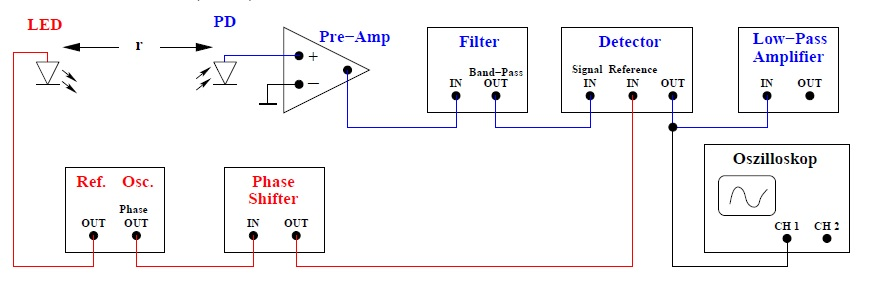
\includegraphics[width=0.8\linewidth]{LEDAufbau.jpg}
	\caption{Aufbau der Photodetektorschaltung. \cite[4]{anleitung303}}
	\label{fig:ledaufbau}
\end{figure}
